\chapter{Projections}

The word "projection" has two main meanings in everyday life. One is a projection as a forecast or estimate of something in the future based on the current situation; another is the result of shining a light to cast a shadow or show a movie. Both these definitions apply to mathematical projection.

Projections are used in many fields, such as science, math, engineering, and finance. Here are a few examples: 
\begin{itemize}
\item Investors evaluate risk and return of a portfolio by projecting an asset’s return onto a reference portfolio.
\item Astronomers analyze the motion of stellar objects by projecting the object’s true motion onto the plane of the sky.
\item Robotics engineers use projections to prevent robots from running into obstacles by projecting the robot’s position onto the optimal path.
\end{itemize}

Mathematically, a projection describes the relationship of one vector to another in terms of direction and orthogonality. Given two vectors, $\mathbf{u}$ and $\mathbf{v}$, the projection of $\mathbf{u}$ onto $\mathbf{v}$ separates $\mathbf{u}$ into two components. The first component signifies how much $\mathbf{u}$ lies in the direction of $\mathbf{v}$. The second signifies the component of $\mathbf{u}$ that is orthogonal (perpendicular) to $\mathbf{v}$. \index{projections} 

The figure~\ref{fig:projection} depicts a projection. The perpendicular line dropped from the end of $\mathbf{u}$ is the \newterm{orthogonal} component. The portion of $\mathbf{u}$ that lies in the direction of $\mathbf{v}$ is the blue segment. 
\index{projections!visualization of}
\begin{figure}[htbp]
    \centering
	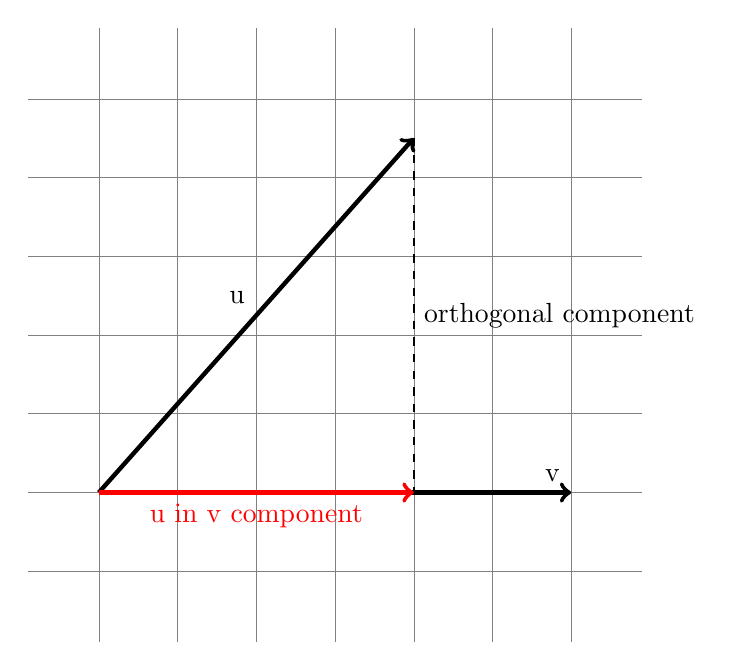
\begin{tikzpicture}
	\draw[step=1cm, gray, very thin](-1.9, -1.9) grid (5.9,5.9);
	\draw[black, ultra thick, ->] (-1,0) -- (3,4.5) node[midway,above left] {u};
	\draw[black, ultra thick, ->] (-1,0) -- (5,0) node[above left] {v};
	\draw[black, thick, dashed] (3,4.5) -- (3,0) node[midway, right] {orthogonal component};
	\draw[red, ultra thick, ->] (-1,0) -- (3,0) node[midway, below] {u in v component};
	\end{tikzpicture}
    \caption{The projection of $u$ onto $v$}
    \label{fig:projection}
\end{figure}

You can also think of a projection as the shadow cast by one vector onto the other by an overhead light. See Figure~\ref{fig:projection2}

\begin{figure}[htbp]
    \centering
	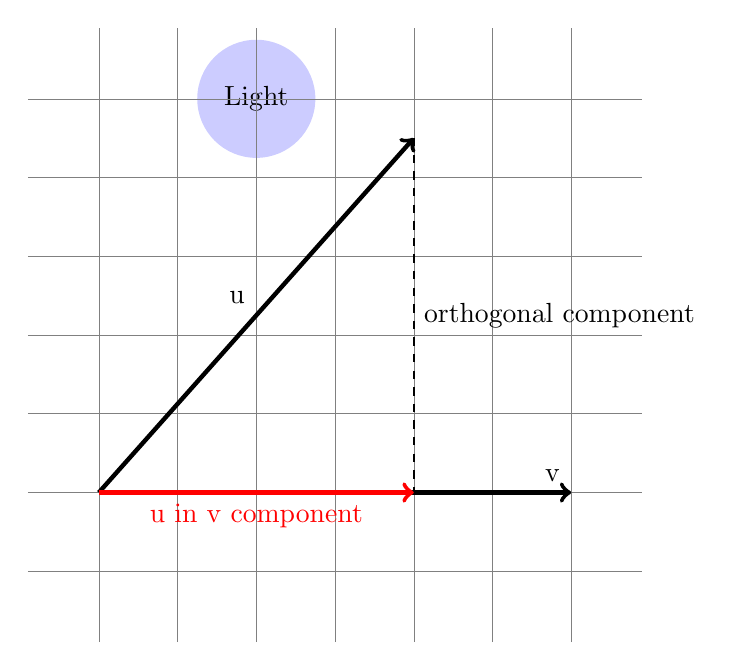
\begin{tikzpicture}[fatnode/.style={circle, fill=blue!20, minimum size=15mm}]
	\node[fatnode] (A) at (1, 5) {Light};
	\draw[step=1cm, gray, very thin](-1.9, -1.9) grid (5.9,5.9);
	\draw[black, ultra thick, ->] (-1,0) -- (3,4.5) node[midway,above left] {u};
	\draw[black, ultra thick, ->] (-1,0) -- (5,0) node[above left] {v};
	\draw[black, thick, dashed] (3,4.5) -- (3,0) node[midway, right] {orthogonal component};
	\draw[red, ultra thick, ->] (-1,0) -- (3,0) node[midway, below] {u in v component};
	\end{tikzpicture}
    \caption{Projection of $u$ onto $v$ with a light included to simulate a shadow.}
    \label{fig:projection2}
\end{figure}

The projected vector can be in any direction and its length can extend beyond the vector onto which it is projecting. See Figure~\ref{fig:projection3}. 

\begin{figure}[htbp]
    \centering
	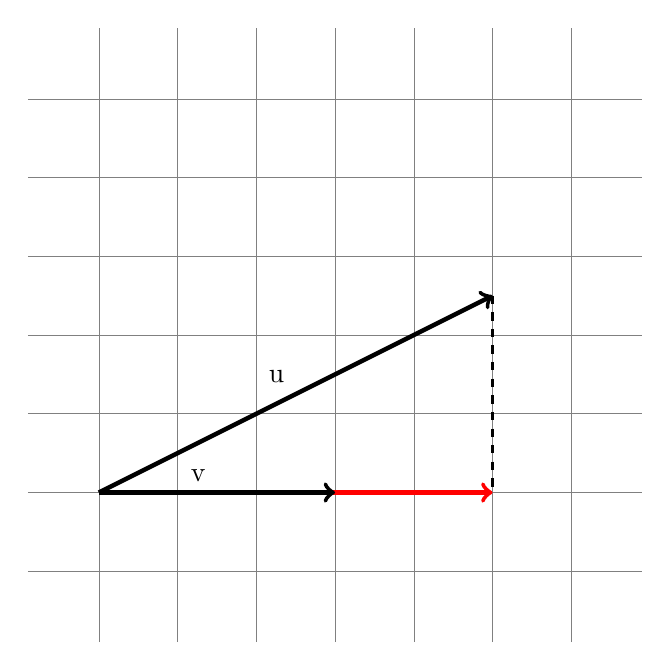
\begin{tikzpicture}  
	\draw[step=1cm, gray, very thin](-1.9, -1.9) grid (5.9,5.9);
	\draw[black, ultra thick, ->] (-1,0) -- (4,2.5)node[midway,above left] {u};
	\draw[red, ultra thick, ->] (-1,0) -- (4,0);
	\draw[black, ultra thick, ->] (-1,0) -- (2,0)node[midway,above left] {v};
	\draw[black, thick, dashed] (4,2.5) -- (4,0);
	\end{tikzpicture}
    \caption{Projection vector extended beyond $v$.}
    \label{fig:projection3}
\end{figure}

To calculate the projection of 
$\mathbf{v}$ onto $\mathbf{u}$, use this formula:
\index{projections!formula for}
\begin{mdframed}[style=important]

$$
\text{Projection of }\mathbf u\text{ onto }\mathbf v:\quad 
\operatorname{proj}_{\mathbf v}(\mathbf u)=\frac{\mathbf u\cdot \mathbf v}{\lVert \mathbf v\rVert^2}\,\mathbf v = \frac{\mathbf u\cdot \mathbf v}{\mathbf{v} \cdot \mathbf{v}}\,\mathbf v
$$
where $\mathbf u\cdot \mathbf v$ is the dot product of $\vec{\mathbf{u}}$ and $\vec{\mathbf{v}}$. Note that either form of the equation works, and the $\mathbf v$ being multiplied by the dot product quotient cannot be cancelled because it is a vector, not a scalar. 
\end{mdframed}
Note that the denominator is the magnitude squared of vector $\mathbf{v}$.
$$\left(\sqrt{a_1^2 + a_2^2 + ... + a_n^2} \right)^{2}$$

You learned previously that this is the same as the dot product of a vector with itself.
$${v\cdot v}$$
In the examples that follow, we will simplify to the dot product notation.

Let's look at a specific example:
$$u = (1,4,6)$$ 
$$v = (-2,6,2)$$ 

$$\mathbf{proj}_\mathbf{v}(\mathbf{u}) = \frac{u\cdot v}{\parallel {v}\parallel ^2}v$$
$$\mathbf{proj}_\mathbf{v}(\mathbf{u}) = \frac{(1,4,6)\cdot(-2,6,2)}{ (-2,6,2)\cdot (-2,6,2)}(-2,6,2)$$
$$\mathbf{proj}_\mathbf{v}(\mathbf{u}) = (\frac{34}{44}(-2,6,2)$$
$$\mathbf{proj}_\mathbf{v}(\mathbf{u}) = (-1.545, 4.64, 1.545)$$

As you work your way through this course, you will have a chance to apply the calculations you learn in this chapter to a variety of problems. Specifically, the next chapter shows how to transform a set of linearly independent vectors into a set of orthogonal ones. Projections are essential to that transformation. 

\begin{Exercise}[title={Projections}, label=projections]
	Find the projection of $\mathbf{a}$ on $\mathbf{b}$ where:
	$$a = (1,3)$$
	$$b = (-4,6)$$
\end{Exercise}
\begin{Answer}[ref=projections]
	Compute dot product of $\mathbf{a}$ and $\mathbf{b}$:
	$$1*-4 + 3*6 = -4 +18 = 14$$
	Compute the dot product of $\mathbf{b}$ and $\mathbf{b}$
	$$16 + 36 = 52 $$
	$$14/52 * (-4,6) = (-1.076 , 1.61)$$
\end{Answer}
 
\section{Projections in Python}

Create a file called \filename{projections.py} and enter this code:
\begin{Verbatim}
import numpy as np

# define two vectors  
a = np.array([1, 4, 6])   
b = np.array([-2, 6, 2])  
  
# use np.dot() to calculate the dot product
projection_a_on_b = (np.dot(a, b)/np.dot(b, b))*b
  
print("The projection of vector a on vector b is:", projection_a_on_b)
\end{Verbatim}
 
\section{Where to Learn More}

Watch this Introduction to Projections from Khan Academy from your digital resources:
\url{https://rb.gy/yf0i3}

